\documentclass[border=5pt]{standalone}
\usepackage{tikz}
\usetikzlibrary{calc}
\usepackage{amsmath}
\begin{document}
    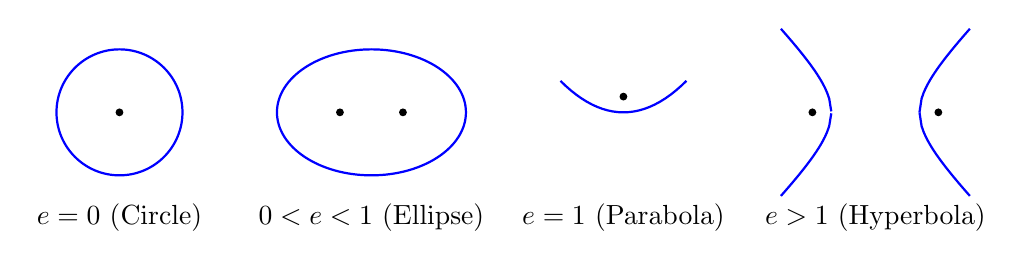
\begin{tikzpicture}[scale=0.8]
        % Draw circle (e = 0)
        \begin{scope}[xshift=-6cm]
            \draw[blue, thick] (0,0) circle (1cm);
            \node[circle, fill, inner sep=1pt] at (0,0) {};
            \node[below] at (0,-1.3) {$e = 0$ (Circle)};
        \end{scope}

        % Draw ellipse (0 < e < 1)
        \begin{scope}[xshift=-2cm]
            \draw[blue, thick] (0,0) ellipse (1.5cm and 1cm);
            \node[circle, fill, inner sep=1pt] at (0.5,0) {};
            \node[circle, fill, inner sep=1pt] at (-0.5,0) {};
            \node[below] at (0,-1.3) {$0 < e < 1$ (Ellipse)};
        \end{scope}

        % Draw parabola (e = 1)
        \begin{scope}[xshift=2cm]
            \draw[blue, thick, domain=-1:1] plot (\x, {0.5*\x*\x});
            \node[circle, fill, inner sep=1pt] at (0,0.25) {};
            \node[below] at (0,-1.3) {$e = 1$ (Parabola)};
        \end{scope}

        % Draw hyperbola (e > 1)
        \begin{scope}[xshift=6cm]
            \draw[blue, thick, domain=0.7:1.5] plot (\x, {sqrt(\x*\x-0.48999)});
            \draw[blue, thick, domain=0.7:1.5] plot (\x, {-sqrt(\x*\x-0.48999)});
            \draw[blue, thick, domain=-1.5:-0.7] plot (\x, {sqrt(\x*\x-0.49)});
            \draw[blue, thick, domain=-1.5:-0.7] plot (\x, {-sqrt(\x*\x-0.49)});
            \node[circle, fill, inner sep=1pt] at (1,0) {};
            \node[circle, fill, inner sep=1pt] at (-1,0) {};
            \node[below] at (0,-1.3) {$e > 1$ (Hyperbola)};
        \end{scope}
    \end{tikzpicture}
\end{document}
